\section{Il significato dell'approssimazione}

\subsection{Intuizione e necessità dell'approssimazione}

Considerando una proprietà semantica concreta di un programma, denotata come
$[\![P]\!]$, e una proprietà target $Q$ che si vuole verificare.
L'obiettivo ideale sarebbe verificare se $[\![P]\!] \subseteq Q$.
Tuttavia, a causa del Teorema di Rice e dell'indecidibilità dell'arresto,
questa inclusione è in generale indecidibile.
Per questo motivo si ricorre a un'approssimazione ${[\![P]\!]}^{\#}$ di $[\![P]\!]$.

\begin{definizione}{Approssimazione}{approximation}

    Per rendere il problema decidibile, si calcola un'approssimazione
${[\![P]\!]}^{\#}$ della semantica concreta $[\![P]\!]$ tale che rispetti due proprietà:
\begin{itemize}
    \item \textbf{Soundness (Correttezza)}: $[\![P]\!] \subseteq {[\![P]\!]}^{\#}$.
    L'approssimazione deve includere tutti i comportamenti reali del
    programma.
    \item \textbf{Decidability (Decidibilità)}: La verifica
    ${[\![P]\!]}^{\#} \subseteq Q$ deve essere decidibile.
\end{itemize}

\end{definizione}

\begin{nota}{L'importanza della soundness}{}

La condizione di soundness è cruciale (\Cref{def:approximation}).
Se si riesce a dimostrare che l'approssimazione è sicura
(${[\![P]\!]}^{\#} \subseteq Q$), allora per la proprietà di transitività
dell'inclusione, è possibile concludere che anche il programma reale è
sicuro ($[\![P]\!] \subseteq Q$).

Tuttavia, se l'approssimazione non soddisfa la proprietà
(${[\![P]\!]}^{\#} \not\subseteq Q$), non è possibile concludere nulla con
certezza; potrebbe trattarsi di un vero bug o di un falso allarme dovuto
all'imprecisione dell'astrazione (``I don't know'').

\end{nota}

\subsection{Astrazione}

\begin{definizione}{Astrazione}{abstraction_def}

L'astrazione è il processo di sostituzione di un oggetto concreto con una
descrizione che si focalizza solo su alcune proprietà di interesse,
ignorandone altre.


Un'astrazione in un dominio di proprietà $\wp(\Sigma)$ di oggetti in $\Sigma$
è un sottoinsieme $A \subseteq \wp(\Sigma)$ tale che:
\begin{itemize}
    \item Gli elementi in $A$ sono descritti con precisione (``senza perdita di precisione'').
    \item Gli elementi non in $A$ devono essere rappresentati (approssimati)
    da elementi di $A$, introducendo una perdita di precisione.
\end{itemize}

\end{definizione}


\subsubsection{Oggetti}

Quando si analizza un programma è necessario considerare oggetti che rappresentano
parti dello stato di esecuzione. Tra questi è possibile includere:
\begin{itemize}
    \item Valori delle variabili (interi, booleani, puntatori, ecc.).
    \item Variabili stesse (nomi, indirizzi, ecc.).
    \item Stack di esecuzione (chiamate di funzione, contesti, ecc.).
    \item Environment (mappature tra variabili e valori).
    \item \ldots
\end{itemize}

\subsubsection{Proprietà e reticolo delle proprietà}

\begin{definizione}{Proprietà}{property_def}
Le proprietà sono insiemi (\Cref{def:set}) di oggetti (valori, variabili, stack, ecc.)
che condividono una certa caratteristica.
\end{definizione}

\begin{esempio}{Esempio di proprietà}{property_example}
Consideriamo il dominio degli interi $\mathbb{Z}$. Una proprietà potrebbe essere
l'insieme dei numeri pari:
\[
P = \{ x \in \mathbb{Z} \mid x \mod 2 = 0 \}
\]
\end{esempio}


\begin{definizione}{Reticolo delle proprietà}{lattice_of_properties}
L'insieme di tutte le possibili proprietà $\wp(\Sigma)$ di oggetti in $\Sigma$
è un reticolo distributivo completo definito come:
\[
\langle \wp(\Sigma), \subseteq, \emptyset, \Sigma, \cup, \cap, \neg \rangle
\]
dove:
\begin{itemize}
    \item Una proprietà è un sottoinsieme di $\Sigma$
    \item L'ordine parziale $\subseteq$ è dato dalle implicazioni logiche tra
    le proprietà.
    \item L'elemento minimo è $\emptyset$ e rappresenta la proprietà falsa
    (nessun oggetto soddisfa la proprietà).
    \item L'elemento massimo è $\Sigma$ e rappresenta la proprietà vera
    (tutti gli oggetti soddisfano la proprietà).
    \item L'operazione di join è l'unione di insiemi ($\cup$).
    \item L'operazione di meet è l'intersezione di insiemi ($\cap$).
    \item La negazione $\neg$ è il complemento rispetto a $\Sigma$
    ($\neg P = \Sigma \setminus P$).
\end{itemize}
\end{definizione}

\subsection{Direzione dell'astrazione}

Quando si approssima una proprietà concreta $P$ con una astratta $P^{\#}$,
è possibile procedere in due direzioni:
\begin{enumerate}
    \item \textbf{Approssimazione dal basso (from below)}: $P^{\#} \subseteq P$.
    \item \textbf{Approssimazione dall'alto (from above)}: $P \subseteq P^{\#}$.
\end{enumerate}


\subsubsection{Approssimazione dal basso}
Nel caso di approssimazione dal basso, $P^{\#} \subseteq P$ se un elemento
appartiene a $P^{\#}$, è certo che appartenga a $P$ (``Yes''), ma se non
appartiene, non sappiamo (``I don't know'').

Questo approccio è utile per dimostrare la presenza di bug (test), ma non la
loro assenza.

\begin{esempio} {Approssimazione dal basso}{approximation_from_below}

Nell'approssimazione dal basso, l'insieme
astratto $P^{\#}$ è contenuto interamente nell'insieme concreto $P$.
Formalmente, vale la relazione:
\[ P^{\#} \subseteq P \]

L'obiettivo è rispondere alla domanda se una coppia $\langle x, y \rangle$
appartiene all'insieme concreto $P$ utilizzando solo l'informazione fornita
dall'approssimazione $P^{\#}$.
In questa configurazione, si presentano due casi distinti:

\begin{itemize}
    \item \textbf{Caso 1: $\langle x, y \rangle \notin P^{\#}$.}
    Se l'elemento non si trova nell'insieme astratto, non si può concludere
    nulla rispetto all'insieme concreto. Potrebbe trovarsi in $P$
    (ma fuori da $P^{\#}$) oppure essere completamente esterno a $P$.
    La risposta è quindi: \textbf{``I don't know''}.

    \item \textbf{Caso 2: $\langle x, y \rangle \in P^{\#}$.}
    Se l'elemento si trova nell'insieme astratto, poiché $P^{\#}$ è un
    sottoinsieme di $P$, si è certi che l'elemento appartenga anche
    all'insieme concreto. La risposta è quindi: \textbf{``Yes''}.
\end{itemize}

Questa tecnica è utile per dimostrare la presenza di una proprietà
(o di un bug), ma non la sua assenza (completezza ma non correttezza nel senso
della verifica formale classica).


\begin{figure}[H]
    \centering
    
\includegraphics[width=0.6\textwidth]{images/th_06/01.png}
    \caption{L'immagine illustra il concetto di approssimazione dal basso,
    dove l'insieme astratto $P^{\#}$ è un sottoinsieme dell'insieme concreto $P$.}
    \label{fig:th_06_01}
\end{figure}

\end{esempio}

\subsubsection{Approssimazione dall'alto}

L'approccio di approssimazione dall'alto, $P \subseteq P^{\#}$,
è la direzione standard per la verifica di sicurezza (safety).
Se un elemento non è in $P^{\#}$, sicuramente non è in $P$ (``No'').
Se è in $P^{\#}$, potrebbe essere in $P$ oppure essere un falso positivo.

\begin{esempio} {Approssimazione dall'alto}{approximation_from_above}

Nell'approssimazione dall'alto, l'insieme astratto $P^{\#}$ è un sovrainsieme
dell'insieme concreto $P$. Formalmente, vale la relazione:
\[ P \subseteq P^{\#} \]

Questa è la forma di approssimazione standard per la verifica di
sicurezza (safety).
L'obiettivo è rispondere alla domanda se una coppia $\langle x, y \rangle$
appartiene all'insieme concreto $P$ utilizzando solo l'informazione fornita
dall'approssimazione $P^{\#}$.
In questa configurazione, si presentano due casi distinti:

\begin{itemize}
    \item \textbf{Caso 1: $\langle x, y \rangle \notin P^{\#}$.}
    Se l'elemento non appartiene all'insieme astratto (che è più grande),
    non può appartenere nemmeno all'insieme concreto $P$.
    La risposta è quindi: \textbf{``No''}.
    Questo è il caso più potente: permette di escludere comportamenti indesiderati con certezza.

    \item \textbf{Caso 2: $\langle x, y \rangle \in P^{\#}$.}
    Se l'elemento appartiene all'insieme astratto, potrebbe appartenere a $P$
    oppure essere un elemento ``spurio'' aggiunto dall'astrazione (un falso
    positivo).
    La risposta è quindi: \textbf{``I don't know''}.
\end{itemize}


\begin{figure}[H]
    \centering
    
\includegraphics[width=0.6\textwidth]{images/th_06/02.png}
    \caption{L'immagine illustra il concetto di approssimazione dall'alto,
    dove l'insieme astratto $P^{\#}$ è un sovrainsieme dell'insieme concreto $P$.}
    \label{fig:th_06_02}
\end{figure}

\end{esempio}

\begin{nota}{Correttezza dell'approssimazione dall'alto}{approximation_direction_choice}

Questo approccio garantisce la correttezza (soundness): se l'analisi dice che
un errore non può verificarsi (non è in $P^{\#}$), allora l'errore non si
verifica davvero nel programma concreto.
\end{nota}

\subsection{Esempi di domini astratti}

L'efficacia dell'analisi dipende dalla scelta del dominio astratto.
Ecco alcuni esempi classici applicati alle variabili intere:

\subsubsection{Dominio dei segni}

Il programma si occupa della manipolazione dei numeri interi e si vuole
studiare le proprietà relative ai segni (positivo, negativo, zero) dei valori
delle variabili.
La semantica concreta si occupa delle operazioni standard che manipolano i valori
interi (somma, sottrazione, ecc.), mentre la semantica astratta si concentra
sulla manipolazione dei segni attraverso regole astratte.

\begin{figure}[H]
    \centering
    
\includegraphics[width=0.4\textwidth]{images/th_06/03.png}
    \caption{L'immagine illustra il dominio astratto dei segni.}
\label{fig:th_06_03}
\end{figure}

Il dominio concreto studiato è $\wp(\mathbb{Z})$ e la proprietà che si vuole
studiare è il segno delle variabili.
Il dominio astratto (\Cref{def:abstraction_def}) dei segni $D^\#$ è costituito
dai seguenti elementi:
\begin{itemize}
    \item $(+)$ che rappresenta i numeri positivi ($> 0$), ovvero l'insieme
    $\{1, 2, 3, \ldots\}$
    \item $(-)$ che rappresenta i numeri negativi ($< 0$), ovvero l'insieme
    $\{-1, -2, -3, \ldots\}$
    \item $(0)$ che rappresenta il numero zero, ovvero l'insieme $\{0\}$
    \item $\bot$ rappresenta l'insieme vuoto $\emptyset$ (nessun valore
    possibile, codice irraggiungibile).
    \item $\top$ rappresenta l'intero insieme $\mathbb{Z}$ (qualsiasi valore
    intero è possibile, ``non so'').
\end{itemize}
\paragraph{Relazione di astrazione}
Un insieme $X$ in $\wp(\mathbb{Z})$ è approssimato dal più piccolo insieme di
interi che contiene $X$ ed è rappresentabile nel dominio dei segni.
Formalmente, questo forma un reticolo completo (\Cref{def:complete_lattice})
dove l'ordine parziale $\sqsubseteq$ riflette l'inclusione insiemistica
delle concretizzazioni.

\begin{figure}[H]
    \centering
    
\includegraphics[width=0.3\textwidth]{images/th_06/04.png}
    \caption{L'immagine illustra il reticolo del dominio dei segni.}
\label{fig:th_06_04}
\end{figure}

Il reticolo rappresentato in \Cref{fig:th_06_04} mostra che gli elementi
$+$, $0$ e $-$ sono incomparabili tra loro, ma sono tutti ``sotto'' $\top$ e
``sopra'' $\bot$.

\begin{nota}{Limitazioni e operazioni astratte}{signs_domain_limitations}
Il dominio dei segni è molto astratto e perde molte informazioni rispetto al
dominio concreto o ad altri domini come gli intervalli.
Le operazioni devono essere ridefinite per lavorare su questi simboli.
Ad esempio:
\begin{itemize}
    \item $(+) + (+) = (+)$ (La somma di due positivi è positiva)
    \item $(+) + (-) = \top$ (La somma di un positivo e un negativo è
    sconosciuta nel dominio dei segni, poiché il risultato dipende dai valori
    assoluti che sono stati astratti).
\end{itemize}
Questo dimostra come l'astrazione garantisca la terminazione e la
decidibilità, pagando il prezzo della precisione (restituendo $\top$ quando
non può determinare un segno preciso).
\end{nota}

\subsection{Approssimazione delle computazioni}

Oltre ad astrarre i dati (valori delle variabili), l'analisi statica astrae
il concetto stesso di esecuzione del programma.

L'obiettivo è passare da una visione basata su singole esecuzioni (vedi
\ref{subsec:trace_semantics}) a una visione basata su insiemi di stati
calcolabili.

\begin{figure}[H]
    \centering
    
\includegraphics[width=0.8\textwidth]{images/th_06/05.png}
    \caption{L'immagine illustra il processo di astrazione delle esecuzioni
    del programma.}
\label{fig:th_06_05}
\end{figure}

Questo processo di astrazione avviene attraverso diversi stadi concettuali
fondamentali:
\begin{itemize}
    \item \textbf{Small-step transition semantics}
    \item \textbf{Computing on sets} (Calcolo su insiemi)
    \item \textbf{Computing by Fixpoint} (Calcolo tramite punto fisso)
    \item \textbf{Collecting semantics} (Semantica collettrice)
\end{itemize}

\subsubsection{Small-step transition semantics}
In questa fase, invece di considerare l'intera storia temporale
continua $x(t)$ di un'esecuzione, viene considerato il comportamento del
programma in singoli passi di transizione.
Questo approccio definisce le regole operazionali (semantica operazionale) che
permettono di passare da uno stato corrente al successivo, creando una
traiettoria discreta di stati.

\begin{figure}[H]
    \centering
    
\includegraphics[width=0.6\textwidth]{images/th_06/06.png}
    \caption{L'immagine illustra la transizione tra stati discreti nel tempo
    durante l'esecuzione di un programma.}
\label{fig:th_06_06}
\end{figure}

\subsubsection{Computing on sets (Calcolo su insiemi)}

Invece di analizzare una singola traiettoria (visualizzabile come un singolo
puntino che si muove nel grafico degli stati nel tempo), l'analisi
considera l'evoluzione di un insieme di stati simultaneamente.
Ad ogni istante discreto, viene considerato l'insieme di tutti i possibili
stati in cui il programma potrebbe trovarsi dato un insieme di stati
iniziali.

\begin{figure}[H]
    \centering
    
\includegraphics[width=0.6\textwidth]{images/th_06/07.png}
    \caption{L'immagine illustra l'evoluzione di un insieme di stati nel
    tempo durante l'esecuzione di un programma.}
\label{fig:th_06_07}
\end{figure}

\subsubsection{Computing by fixpoint (Calcolo tramite punto fisso)}

Per calcolare l'insieme di tutti gli stati raggiungibili (che potrebbero
evolvere all'infinito nel tempo), viene utilizzato un approccio iterativo.
Partendo dagli stati iniziali (spesso $\bot$ o l'insieme degli stati di
ingresso) (vedi \ref{fig:th_06_08}) viene applicata ripetutamente la funzione
di transizione all'interno dell'insieme.

\begin{figure}[H]
    \centering
    
\includegraphics[width=0.6\textwidth]{images/th_06/08.png}
    \caption{L'immagine illustra lo stato iniziale dell'iterazione per il
    calcolo del punto fisso.}
\label{fig:th_06_08}
\end{figure}

L'insieme degli stati accumulati cresce (vedi \ref{fig:th_06_09}) fino a
quando non si stabilizza, ovvero quando un'ulteriore applicazione della
funzione non aggiunge nuovi stati.

\begin{figure}[H]
    \centering
    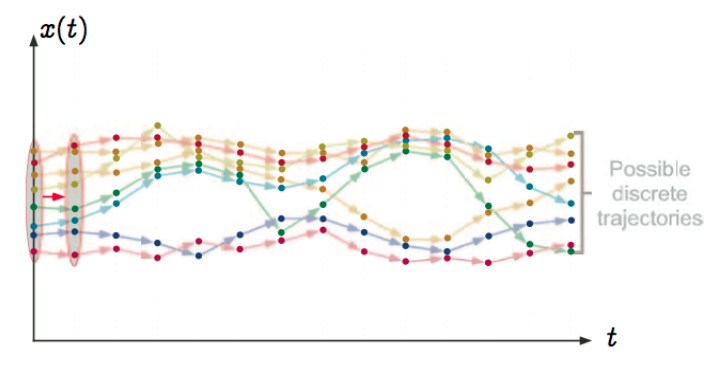
\includegraphics[width=0.6\textwidth]{images/th_06/09.png}
    \caption{L'immagine illustra l'espansione progressiva dell'insieme degli
    stati raggiungibili attraverso l'applicazione iterativa della funzione di
    transizione.}
\label{fig:th_06_09}
\end{figure}

Questo stato stabile (vedi \ref{fig:th_06_10}) è il punto fisso (vedi
\ref{subsec:fixpoint}).

\begin{figure}[H]
    \centering
    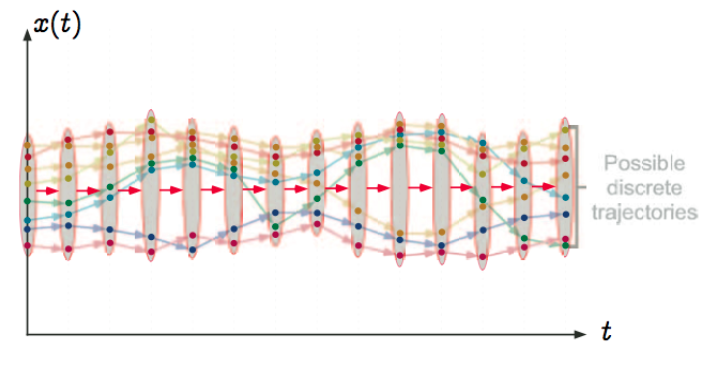
\includegraphics[width=0.6\textwidth]{images/th_06/10.png}
    \caption{L'immagine illustra il raggiungimento del punto fisso: l'insieme
    degli stati si è stabilizzato e include tutte le possibili traiettorie
    discrete.}
\label{fig:th_06_10}
\end{figure}


\subsubsection{Collecting semantics (Semantica collettrice)}
La semantica collettrice associa ad ogni punto del programma l'insieme di
tutti gli stati che possono essere raggiunti in quel punto durante qualsiasi
esecuzione senza tenere conto dell'ordine temporale (questa è già una
astrazione).

\begin{figure}[H]
    \centering
    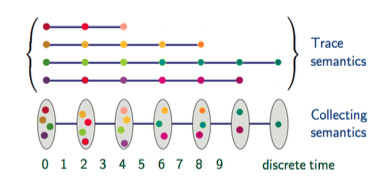
\includegraphics[width=0.5\textwidth]{images/th_06/11.png}
    \caption{L'immagine illustra la semantica collettrice che associa insiemi di
    stati ai punti del programma.}
\label{fig:th_06_11}
\end{figure}


\begin{nota}{Introduzione di rumore}{noise_intro}

Il passaggio alla semantica collettrice introduce ``rumore'' o approssimazione.
Associando gli stati ai punti di programma (es. riga di codice) e non al
tempo, potrebbe includere percorsi spuri (spurious traces) che saltano tra
stati validi in modi che l'esecuzione reale non farebbe, sebbene rimanga
limitato agli stati raggiungibili.

\begin{figure}[H]
    \centering
    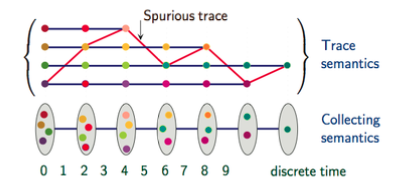
\includegraphics[width=0.5\textwidth]{images/th_06/12.png}
    \caption{L'immagine illustra l'introduzione di rumore nella semantica
    collettrice a causa della perdita di informazioni temporali.}
\label{fig:th_06_12}
\end{figure}

\end{nota}

L'analisi statica procede quindi:
\begin{itemize}
    \item Considerando proprietà (insiemi) di stati invece di stati concreti.
    \item Calcolando su insiemi (approssimando la semantica delle tracce).
    \item Utilizzando la collecting semantics sui punti di programma.
\end{itemize}

Così facendo però rimane ancora il problema della indecidibilità, poiché gli
insiemi di stati possono essere infiniti e non calcolabili.
Infatti è necessario approssimare ulteriormente questi insiemi.

\subsubsection{Computing on properties (Calcolo su proprietà)}

Il calcolo esatto sugli insiemi di stati nella semantica
collettrice è spesso indecidibile o computazionalmente intrattabile (gli insiemi
possono essere infiniti o estremamente complessi).

Per risolvere questo problema, viene introdotta un'ulteriore astrazione;
invece di propagare l'esatto insieme di stati concreti, si calcolano
delle proprietà astratte che sovrapprossimano tali insiemi.

\begin{figure}[H]
    \centering
    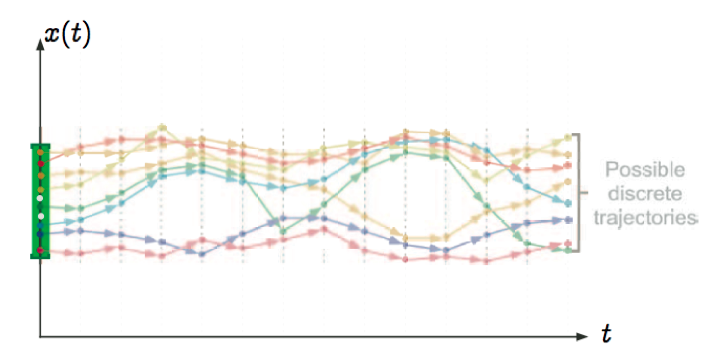
\includegraphics[width=0.6\textwidth]{images/th_06/13.png}
    \caption{L'immagine illustra l'astrazione dei dati: un insieme di stati
    concreti (i punti colorati all'istante iniziale) viene sostituito da una
    singola proprietà astratta (l'intervallo verde) che li include tutti.}
\label{fig:th_06_13}
\end{figure}

In questa fase:
\begin{itemize}
    \item Si sostituiscono gli insiemi di stati concreti con elementi di un
    dominio astratto (es. Segni, Intervalli, Poliedri).
    \item Le operazioni del programma vengono sostituite da operazioni astratte
    che lavorano su queste proprietà.
\end{itemize}


\begin{figure}[H]
    \centering
    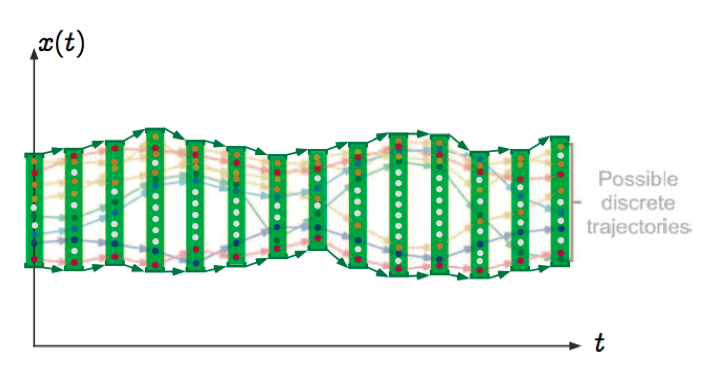
\includegraphics[width=0.6\textwidth]{images/th_06/14.png}
    \caption{L'immagine illustra l'esecuzione astratta: la
    computazione non avviene più sui singoli stati, ma evolve trasformando la
    proprietà astratta (la sequenza di intervalli verdi) passo dopo passo,
    garantendo di coprire tutte le possibili traiettorie discrete.}
\label{fig:th_06_14}
\end{figure}


\begin{nota}{Aggiunta di rumore}{adding_noise}
Questo passaggio introduce ulteriore rumore (perdita di precisione).
Ad esempio, un insieme di stati concreti sparsi potrebbe essere
sovrapprossimato da un singolo intervallo astratto che include anche stati
non spuri.
\end{nota}

\subsection{Gerarchia delle semantiche come astrazioni}

È possibile visualizzare l'intero processo di costruzione dell'analisi statica
come una gerarchia di astrazioni successive, dove ogni livello riduce la
precisione per guadagnare trattabilità o focalizzarsi su proprietà specifiche.

Le figure seguenti mostrano come, partendo dalla stessa realtà concreta, si
possano derivare astrazioni diverse.

\begin{figure}[H]
    \centering
    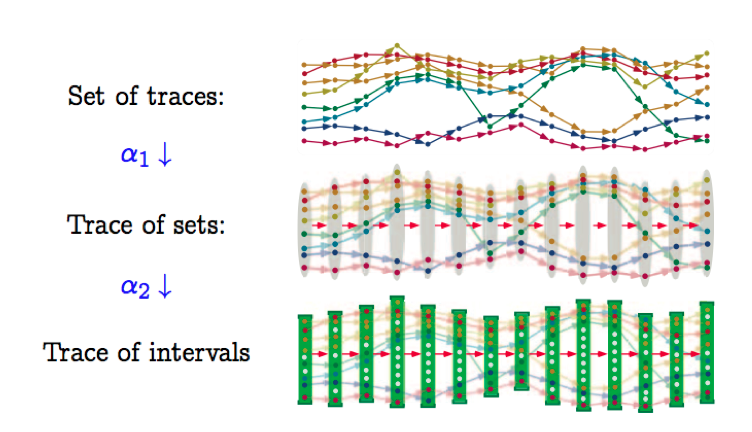
\includegraphics[width=0.6\textwidth]{images/th_06/15.png}
    \caption{Astrazione dei dati ($\alpha_2$): dalle tracce concrete agli
    intervalli, mantenendo la distinzione temporale.}
\label{fig:th_06_15}
\end{figure}

\begin{figure}[H]
    \centering
    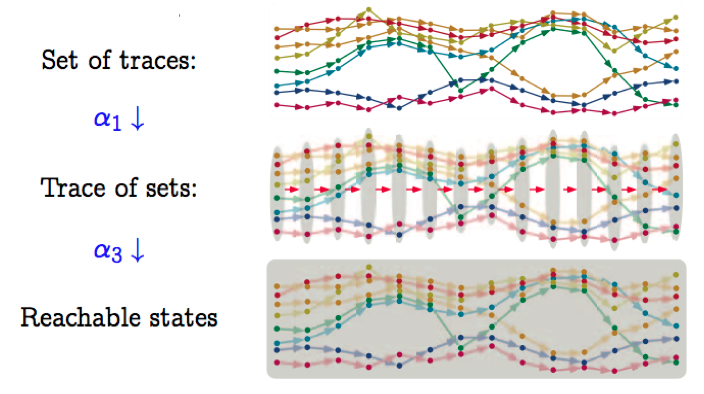
\includegraphics[width=0.6\textwidth]{images/th_06/16.png}
    \caption{Astrazione degli stati raggiungibili ($\alpha_3$): dalle tracce
    concrete all'insieme globale degli stati visitati.}
\label{fig:th_06_16}
\end{figure}

La gerarchia si compone dei seguenti livelli:

\begin{enumerate}
    \item \textbf{Set of traces (Insieme di tracce)}:
    Rappresenta la realtà completa del programma (semantica concreta).
    Distingue ogni singola esecuzione e ogni singolo istante temporale.
    È la massima precisione possibile, ma il calcolo è generalmente impossibile.

    \item \textbf{Trace of sets (Traccia di insiemi) [$\alpha_1$]}:
    Ottenuta tramite la prima astrazione (semantica collettrice).
    Qui si raggruppano le esecuzioni diverse: invece di seguire singole linee,
    si considerano "fasci" (insiemi) di stati per ogni istante discreto.
    Si perde la relazione tra uno stato specifico al tempo $t$ e il suo
    successore al tempo $t+1$, mantenendo solo l'insieme dei possibili stati
    in $t$ e in $t+1$.

    \item \textbf{Ulteriori astrazioni [$\alpha_2$ vs $\alpha_3$]}:
    A partire dalla traccia di insiemi, possiamo astrarre in modi diversi a
    seconda dello scopo:
    \begin{itemize}
        \item \textbf{Trace of intervals ($\alpha_2$ - Figura \ref{fig:th_06_15})}:
        Si applica un'astrazione sui \textbf{dati}. Invece di insiemi di punti
        sparsi, si usano domini astratti geometrici (come gli intervalli
        verdi) per inglobare tutti i valori possibili a ogni passo. Mantiene
        la struttura temporale discreta.
        \item \textbf{Reachable states ($\alpha_3$ - Figura \ref{fig:th_06_16})}:
        Si astrae la dimensione \textbf{temporale}. Invece di distinguere cosa
        accade al passo 1, 2 o 3, si calcola l'unico grande insieme (l'area
        grigia) che contiene tutti gli stati che il programma può raggiungere
        in qualsiasi momento della sua esecuzione.
    \end{itemize}
\end{enumerate}
